\newpage

\section{Problem description \& Hypothesis}
As we can see in the state-of-the-art section, we can extract knowledge from a mobile communication datasets, therefore in this paper the solution is built on the hypotesis of mobility patterns to predict common and well-know, geographical and time based patterns to manage roads and infrastructures in a correlated way with the results figured out.
\\
\\
The figure below shows a theoretical commuting model proposed like a main pattern. 
\\
Two peaks are modeled, $p_1$ in the range $[7, 8]$ and $p_2$ in $[17, 18]$. This first approach to modelize this dynamic set up the two peaks $p_1, p_2$ with the same weight, however, numerical results will show that the weight of each peak depends of the day of the week. A central valley is defined between $[9, 16]$, with a uniform displacement distribution.
\\
An ad-hoc mathematical model is defined in the next section in order to confirm this hypothesis; focusing, filtering and processing the main data to contrast the hypothesis.
\\
\\
The main idea behind the two main peaks in the model, $p_1, p_2$ and the central valley, is that people perform great displacement distances early in the morning i.e.: $p_1$ related with the common business activity. After the first peak $p_1$, people resides in this target destinations, working, eating, etc ..., but in a more static point of view and always performing displacements. The last point in the hypothesis approach showed by Figure~\ref{fig:commuting} is in the second peak $p_2$, when people return to his destination or the last business activites are realized.
\\
\\
The geographical behaviur of the dynamic, always mixed with the temporal component, will by contrasted by means of GIS tools in order to visualize the expansion and contraction in the main points that hypothesys shows: $p_1, p_2$ and the central valley. Exapansion when maximum displacement is reached on the first peak $p_1$ and contraction, but not quite,  when the central valley is reached. Another displacement expansion when peak $p_2$ is reached and its corresponding contraction when among $p_2$ is declining.


 
 \begin{figure}[h]
\begin{center}
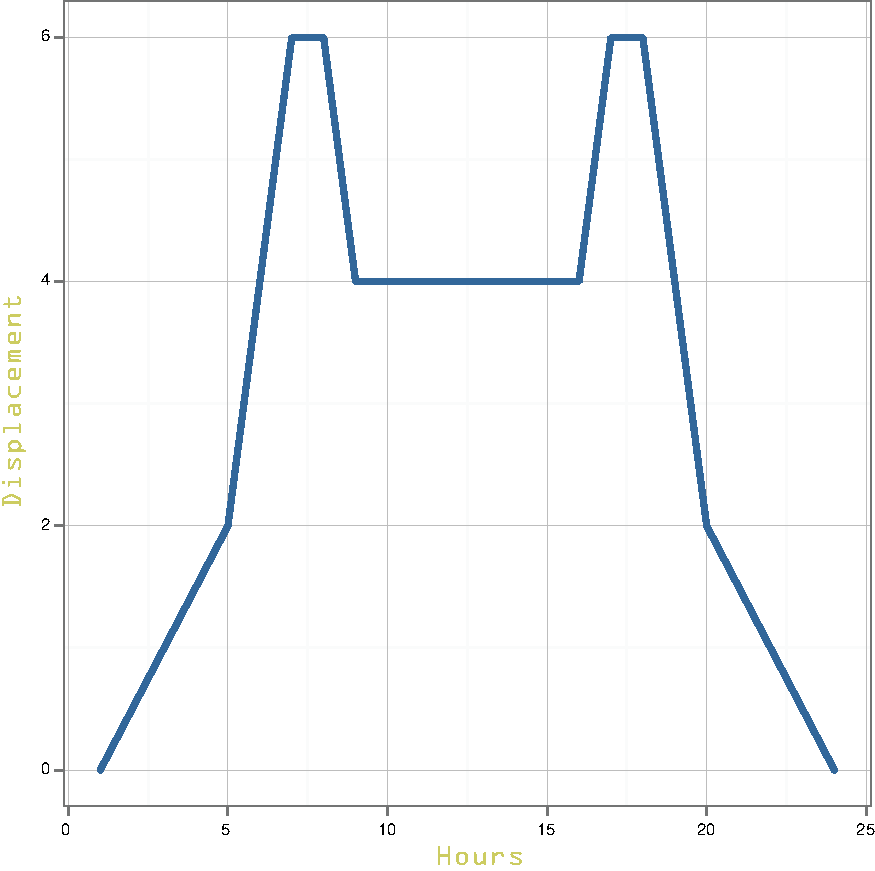
\includegraphics[scale =0.6] {results/images/common_commuting_model.pdf}
\caption{Theoretical Commuting Model}
\label{fig:commuting}
\end{center}
\end{figure}